\begin{figure*}[!t]
    \centering
    \includegraphics[width=0.98\textwidth]{figures/fig02_architecture.pdf}
    \caption{ForceDelta-VLA architecture. Offline, paired force-conditioned and force-agnostic queries of a frozen teacher construct targets for force and delay correction. Online, a shared correction policy maps the cached task context, current wrench history and state, aligned base-action segment, and timing features to two $K$-step corrections. The corrections are added asynchronously to the cached base pose; its gripper command remains unchanged.}
    \label{fig:network_structure}
\end{figure*}

\subsection{Problem Formulation}
\label{sec:problem}

We consider an offline dataset $\mathcal D$ of teleoperated manipulation trajectories. At time $t$, each trajectory provides visual observations $V_t$, a language instruction $L$, robot state $S_t$, demonstrated action $A_t^*$, and the causal wrench history
\begin{equation*}
    \mathcal F_t=\{(s,\mathbf w(s))\mid t-T_F\leq s\leq t\},
\end{equation*}
where $T_F$ is the history duration and $\mathbf w(s)=[\mathbf f(s);\boldsymbol\tau(s)]\in\mathbb R^6$ is the per-arm external end-effector wrench. Pose actions and wrench measurements use the corresponding robot-base frame. A force-conditioned teacher $T_\theta$ maps $(V_t,L,S_t,\mathcal F_t)$ to an $H$-step action chunk relative to $S_t$. Pose actions and corrections below use its normalized pose-action coordinates, with differences scaled by the action standard deviations.

Let $\mathcal P(\cdot)$ extract the pose component of an action. We decompose the commanded pose into a base action and two learned corrections,
\begin{equation}
    \mathcal P(A^{\mathrm{cmd}})
    =\mathcal P(A^{\mathrm{base}})
      +\Delta\hat A^{\mathrm{force}}
      +\Delta\hat A^{\mathrm{delay}}.
    \label{eq:action_comp}
\end{equation}
The force correction models the change induced by the wrench history. The delay correction accounts for the mismatch between the cached base action and a current force-agnostic prediction after expressing both relative to the base-action query state. Both terms modify only pose; the gripper command is inherited from the base action.

Here $\mathcal P(A)=[p;r]$ contains translation $p\in\mathbb R^3$ and a continuous 6D rotation representation $r\in\mathbb R^6$~\cite{zhou2020continuityrotationrepresentationsneural}. Translation is added directly; rotational corrections are added in the teacher's 6D action coordinates and mapped to a valid rotation matrix by Gram--Schmidt orthogonalization. On the bimanual platform, $\mathcal P(A)$, $S_t$, and $\mathcal F_t$ concatenate the corresponding per-arm quantities, so the pose-action dimension doubles and a single correction query predicts both arms jointly. Correction construction is component-wise over the concatenated pose vector; deployment applies the same per-coordinate bound specification independently to each arm.

\subsection{Method Overview}
\label{sec:method_overview}

Training proceeds in three stages (Fig.~\ref{fig:network_structure}). First, we train a temporal force-conditioned VLA teacher. Second, we freeze the teacher and learn a force-agnostic mode that supplies the base action. Third, we freeze both modes, construct force- and delay-correction targets under cached context, and train the correction policy.

\subsection{Force-Conditioned Teacher and Base-Action Mode}
\label{sec:teacher_and_missing}

\subsubsection{Temporal force-conditioned teacher}

We build $T_\theta$ on ForceVLA~\cite{yu2025forcevlaenhancingvlamodels} and replace its instantaneous force embedding with a FAVLA-style causal temporal convolutional network (TCN)~\cite{li2026favlaforceadaptivefastslowvla} that encodes the wrench history,
\begin{equation}
    z_t^F=E_T^F(\mathcal F_t).
    \label{eq:teacher_tcn}
\end{equation}
The teacher is trained on $\mathcal D$ to predict
\begin{equation}
    A_{T,t,1:H}^{\mathrm{cond}}
    =T_\theta(V_t,L,S_t,z_t^F;\epsilon),
    \label{eq:conditioned_teacher}
\end{equation}
where $\epsilon$ is the initial flow noise. We freeze $\theta$ after training.

\subsubsection{Force-agnostic base-action mode}

We distinguish an unavailable wrench history from a physically measured zero wrench. The learned force-agnostic mode represents the former: it replaces the wrench history with a learned token $z_{\varnothing F}$ and a rank-$\rho$ adapter $(W_{\mathrm{in}},W_{\mathrm{out}})$. We collect its trainable parameters as $\phi=\{z_{\varnothing F},W_{\mathrm{in}},W_{\mathrm{out}}\}$. The adapter modifies the pose channels of the action expert,
\begin{equation}
    v^p\leftarrow v^p+W_{\mathrm{out}}\,
    \sigma(W_{\mathrm{in}}h),
    \label{eq:missing_force_adapter}
\end{equation}
where $h$ is an action-expert hidden state, $v^p$ its pose-channel flow output, and $\sigma$ a pointwise nonlinearity. The adapter is active only in the force-agnostic mode. With $\theta$ fixed, optimizing $\phi$ under the teacher's original flow-matching objective defines the base-action operating point.
The resulting base-action prediction is
\begin{equation}
    A_{T,t,1:H}^{\mathrm{base}}
    =T_{\theta,\phi}^{\mathrm{base}}
      (V_t,L,S_t,z_{\varnothing F};\epsilon).
    \label{eq:teacher_missing}
\end{equation}

\subsection{State-Consistent Dual-Correction Distillation}
\label{sec:distillation}

\subsubsection{Correction targets}
\label{sec:teacher_differencing}

For a schedule-replay sample $(t,k)$, let $E_k$ be the visual--language prefix produced from $(V_k,L)$ when base-action query $k$ starts at $t_k$ from state $S_k$ with flow noise $\epsilon_k$. Its force-agnostic action chunk defines the timestamped base action, $A_k^{\mathrm{base}}=A_{T,k}^{\mathrm{base}}$. To match the information available to the deployed correction pathway, target generation reuses $E_k$ while updating the robot state and force history to time $t$:
\begin{align}
    A_{T,t|k,1:K}^{\mathrm{cond}}
    &=T_\theta(E_k,S_t,z_t^F;\epsilon_k)_{1:K},
    \label{eq:cached_conditioned_teacher}\\
    A_{T,t|k,1:K}^{\mathrm{base}}
    &=T_{\theta,\phi}^{\mathrm{base}}
      (E_k,S_t,z_{\varnothing F};\epsilon_k)_{1:K}.
    \label{eq:cached_missing_teacher}
\end{align}
Here $T(E_k,\cdot)$ reuses the cached prefix without encoding a current image. The cached base action and the two current teacher queries share $E_k$ and $\epsilon_k$. For $j=1,\ldots,K\leq H$, the teacher-defined force-correction target is
\begin{equation}
    \Delta A_{T,t|k,j}^{\mathrm{force}}
    =\mathcal P\!\left(A_{T,t|k,j}^{\mathrm{cond}}\right)
     -\mathcal P\!\left(A_{T,t|k,j}^{\mathrm{base}}\right),
    \label{eq:force_target}
\end{equation}
which supervises the force-correction head.

The correction query predicts $K$ action samples at $t_j=t+(j-1)/f_A$, where $f_A$ is the action-sample rate within a chunk. Let $\widetilde S^{p}$ denote the normalized pose coordinates (nine per arm), and let $\sigma_S^{p}$ and $\sigma_A^{p}$ denote the corresponding training-set standard deviations. The cached-state gap is converted to normalized action coordinates as
\begin{equation}
    \Gamma(S_t,S_k)
    =\frac{\sigma_S^{p}+\varepsilon}{\sigma_A^{p}+\varepsilon}
      \odot(\widetilde S_t^{p}-\widetilde S_k^{p}),
    \qquad \varepsilon=10^{-6}.
    \label{eq:coordinate_rebasing}
\end{equation}
The learned delay-correction target is
\begin{equation}
    \Delta A_{T,k\rightarrow t,j}^{\mathrm{delay}}
    =\mathcal P\!\left(A_{T,t|k,j}^{\mathrm{base}}\right)
      -\mathcal P\!\left(A_k^{\mathrm{base}}(t_j)\right)
      +\Gamma(S_t,S_k).
    \label{eq:delay_target}
\end{equation}
Let $\mathcal R(S,a)$ convert a relative action $a$ based at state $S$ into an absolute robot command. The paired targets align the two coordinate bases stepwise:
\begin{equation}
\begin{aligned}
    &\mathcal R\!\left(S_k,\mathcal P(A_k^{\mathrm{base}}(t_j))
      +\Delta A_{T,t|k,j}^{\mathrm{force}}
      +\Delta A_{T,k\rightarrow t,j}^{\mathrm{delay}}\right)\\[-2pt]
    &\qquad\approx\mathcal R\!\left(S_t,
      \mathcal P(A_{T,t|k,j}^{\mathrm{cond}})\right).
\end{aligned}
    \label{eq:absolute_command_equivalence}
\end{equation}
Before clipping, substitution recovers the force-conditioned chunk expressed relative to $S_k$. Since state and action are converted to the same translation-plus-6D representation before component-wise delta construction, the rebasing identity is exact in that representation up to $\varepsilon$; Gram--Schmidt projection is applied after restoring the action delta.

\subsubsection{Correction policy}
\label{sec:residual_policy}

Each base-action query caches a compact representation of its visual--language context. Let $m_k$ denote the validity mask over tokens in $E_k$ from available image views and non-padding language positions; state, force, and action tokens are excluded from $E_k$. Masked mean pooling produces the cached context $(\bar E_k,\bar m_k)$, and the correction policy applies a learned query projector,
\begin{align}
    (\bar E_k,\bar m_k)
    &=\operatorname{Pool}_{M}(E_k,m_k),\nonumber\\
    Z_k^{\mathrm{ctx}}
    &=P_{\mathrm{ctx}}(\bar E_k,\bar m_k).
    \label{eq:context_projection}
\end{align}
Here $\operatorname{Pool}_{M}$ partitions the padded prefix into contiguous, approximately equal-width positional bins and applies masked mean pooling within each bin, retaining the bin-validity mask $\bar m_k$. The projector $P_{\mathrm{ctx}}$ uses $Q$ learned queries to aggregate the valid pooled tokens. We use $M=16$ bins and $Q=2$ learned queries.
The task-context tokens represent the visual--language context available when base-action query $k$ starts. Together, $A_k^{\mathrm{base}}$, $(\bar E_k,\bar m_k)$, and $S_k$ form the timestamped base-action update for query $k$; the latest available update is cached for the correction pathway. The correction policy treats this context as locally valid within a base-action interval. Timestamp-based interpolation provides the aligned segment $A_k^{\mathrm{base}}(t_{1:K})$. A causal encoder maps $\mathcal F_t$ to $u_t^F$. Cache age and interpolation phase are encoded as
\begin{equation}
    \xi_{t,k}=
    \left[\min\!\left(\frac{t-t_k}{c},1\right);\alpha_{t,k}\right],
    \label{eq:time_features}
\end{equation}
where $c=0.6$~s is the age scale and $\alpha_{t,k}$ is the position of $t$ between adjacent base-action samples. The conditioning set is
\begin{align}
    \mathcal C_t=[&P_Z(Z_k^{\mathrm{ctx}});u_t^F;P_S(S_t);
    \nonumber\\[-2pt]
    &P_A(\operatorname{vec}(A_k^{\mathrm{base}}(t_{1:K})));P_\xi(\xi_{t,k})].
    \label{eq:conditioning_set}
\end{align}
Here $P_Z,P_A,P_S$, and $P_\xi$ project to the shared token width; $P_A$ maps the flattened aligned segment to one base-action token. There is no positional encoding: a learned type embedding identifies each condition, so the correction-query output is invariant to permutations of the condition tokens together with their type embeddings. Let $\mathcal C_t^{\mathrm{maskF}}=\operatorname{Mask}_F(\mathcal C_t)$ be the same set with the force token masked.

An attention block $\Phi$ and learned query $q_{\mathrm{corr}}$ predict two $K$-step corrections,
\begin{align}
    \Delta\hat A^{\mathrm{force}}_{t,1:K}
    &=W_{\mathrm{force}}\Phi([\mathcal C_t;q_{\mathrm{corr}}])[q_{\mathrm{corr}}],
    \label{eq:force_output}\\
    \Delta\hat A^{\mathrm{delay}}_{t,1:K}
    &=W_{\mathrm{delay}}
      \Phi([\mathcal C_t^{\mathrm{maskF}};q_{\mathrm{corr}}])[q_{\mathrm{corr}}].
    \label{eq:delay_output}
\end{align}
The mask prevents direct dependence of the delay-correction output on the force token. The two passes share $\Phi$ and use separate output projections.

\subsubsection{Asynchronous schedule replay}
\label{sec:async_training}

We sample an asynchronous schedule before cached-context target extraction and replay the resulting fixed schedule during correction-policy optimization. Inter-query periods are sampled independently as $T_i\sim\mathcal U(1/15,1/5)$~s and base-action-query latencies as $L_i\sim\mathcal U(0.05,0.30)$~s. Query rows are selected greedily on the recorded $30$~Hz state--action time grid according to $T_i$; the selected query timestamps then receive jitter $J_i\sim\mathcal U(-0.01,0.01)$~s to exercise off-grid base-action interpolation. Training instants follow the recorded state--action timestamps, while $\mathcal F_t$ retains all wrench samples in the causal window. If $t_i$ and $\bar t_i=t_i+L_i$ are the start and availability times of query $i$, the active base-action index is
\begin{equation*}
    k(t)=\arg\max_{i:\bar t_i\leq t}t_i.
\end{equation*}
The active base-action update supplies the cached pooled context, aligned base-action segment, and timestamps used to compute the temporal features and stepwise targets. The schedule determines the base-action age, interpolation phase, and base-action-query latency represented during optimization.

With normalized temporal weights $w_j\propto\beta^{j-1}$, $0<\beta\leq1$, and normalized-coordinate mean-squared loss $\ell_{\mathrm{pose}}$, the distillation objective is
\begin{align}
    \mathcal L_{\mathrm{distill}}=\sum_{j=1}^{K}w_j\big[&
      \ell_{\mathrm{pose}}(\Delta\hat A^{\mathrm{force}}_{t,j},
        \Delta A^{\mathrm{force}}_{T,t|k,j})
    \nonumber\\[-2pt]
      &+\lambda_{\mathrm{delay}}
        \ell_{\mathrm{pose}}(\Delta\hat A^{\mathrm{delay}}_{t,j},
        \Delta A^{\mathrm{delay}}_{T,k\rightarrow t,j})\big].
    \label{eq:correction_loss}
\end{align}
The coefficient $\lambda_{\mathrm{delay}}$ balances force-conditioning and delay-correction supervision.

\subsection{Independent Correction Execution}
\label{sec:execution}

The base-action and correction workers execute independently (Fig.~\ref{fig:async_deployment}). Each correction query reads the latest completed base-action update available at its start, together with the current state and $\mathcal F_t$. The resulting $K$-step correction chunk continues using that same cached update throughout its execution; a newly completed base action is adopted by the next correction query.

\begin{figure*}[t]
    \centering
    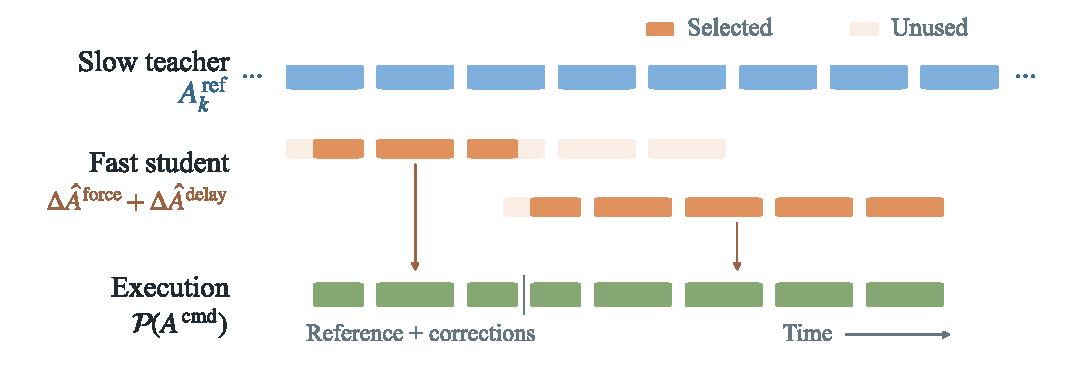
\includegraphics[width=0.82\textwidth]{figures/fig03_async_execution.pdf}
    \caption{Illustrative asynchronous execution with $K=5$. Correction queries read the latest completed base action at their start and retain it for command composition. A newly published correction chunk replaces the preceding chunk; numbered blocks show its active steps. Colors identify base-action updates, and dotted lines mark correction-query completion.}
    \label{fig:async_deployment}
\end{figure*}

Expired correction steps are skipped, and the remaining steps execute sequentially without interpolation. The base pose is interpolated by timestamp. The force and state-consistent delay corrections are bounded independently, added to the base action in normalized delta-action coordinates, and converted to an absolute command using the base-action query state. The supervised delay-correction target already includes $\Gamma(S_t,S_k)$.
